% CollisionalDarkMatter.tex 
%
% Based in the LaTeX template for creating an MNRAS paper
%
% v3.0 released 14 May 2015
% (version numbers match those of mnras.cls)
%
% Copyright (C) Royal Astronomical Society 2015
% 
% Created by Keith T. Smith (Royal Astronomical Society)

% Change log
%
%%%%%%%%%%%%%%%%%%%%%%%%%%%%%%%%%%%%%%%%%%%%%%%%%%
% Basic setup. Most papers should leave these options alone.
\documentclass[fleqn,usenatbib]{mnras}

% MNRAS is set in Times font. If you don't have this installed (most LaTeX
% installations will be fine) or prefer the old Computer Modern fonts, comment
% out the following line
\usepackage{newtxtext,newtxmath}
% Depending on your LaTeX fonts installation, you might get better results with one of these:
%\usepackage{mathptmx}
%\usepackage{txfonts}

% Use vector fonts, so it zooms properly in on-screen viewing software
% Don't change these lines unless you know what you are doing
\usepackage[T1]{fontenc}
\usepackage{ae,aecompl}


%%%%% AUTHORS - PLACE YOUR OWN PACKAGES HERE %%%%%

% Only include extra packages if you really need them. Common packages are:
\usepackage{graphicx}	% Including figure files
\usepackage{amsmath}	% Advanced maths commands
\usepackage{amssymb}	% Extra maths symbols
\usepackage{physics}	% Easy use of common notation.

%\usepackage{quotmark} %Temporal, en lo que soluciono las comillas.
%%%%%%%%%%%%%%%%%%%%%%%%%%%%%%%%%%%%%%%%%%%%%%%%%%

%%%%% AUTHORS - PLACE YOUR OWN COMMANDS HERE %%%%%

% Please keep new commands to a minimum, and use \newcommand not \def to avoid
% overwriting existing commands. Example:
%\newcommand{\pcm}{\,cm$^{-2}$}	% per cm-squared
\newcommand{\f}[1][t]{f(\vb*{r},\vb*{v};#1)}
\newcommand{\dens}[1][t]{\rho(\vb*{r};#1)}
\newcommand{\acce}[1][t]{\vb*{a}(\vb*{r};#1)}
\newcommand{\pot}[1][t]{\Phi(\vb*{r};#1)}

\newcommand{\rv}{\vb*{r},\vb*{v}}
\newcommand{\crosssection}{\langle \sigma v \rangle}
\newcommand{\toInt}[1]{\ensuremath{\lfloor#1\rceil}}
%TODO borrar los comandos no usados.

%%%%%%%%%%%%%%%%%%%%%%%%%%%%%%%%%%%%%%%%%%%%%%%%%%

%%%%%%%%%%%%%%%%%%% TITLE PAGE %%%%%%%%%%%%%%%%%%%

% Title of the paper, and the short title which is used in the headers.
% Keep the title short and informative.
%\title[Short title, max. 45 characters]{Simulating collisional dark matter using a Lattice Boltzmann method}

\title[Collisional lattice dynamics]{Lattice dynamics for a collisional dark matter fluid}
%\title[Collisional lattice dynamics]{Lattice dynamics for a collisional stellar fluid}



% The list of authors, and the short list which is used in the headers.
% If you need two or more lines of authors, add an extra line using \newauthor
\author[J. A. Acevedo-Barroso \& J. E. Forero-Romero]{
Javier A. Acevedo-Barroso,$^{1}$\thanks{E-mail: ja.acevedo12@uniandes.edu.co}
Jaime E. Forero-Romero,$^{1}$\thanks{E-mail: je.forero@uniandes.edu.co}
\\
% List of institutions
$^{1}$Departamento de F\'isica, Universidad de los Andes, Cra. 1 No. 18A-10 Edificio Ip, CP 111711, Bogot\'a, Colombia\\
}

% These dates will be filled out by the publisher
\date{Accepted XXX. Received YYY; in original form ZZZ}

% Enter the current year, for the copyright statements etc.
\pubyear{2019}

% Don't change these lines
\begin{document}
\label{firstpage}
\pagerange{\pageref{firstpage}--\pageref{lastpage}}
\maketitle

% Abstract of the paper
\begin{abstract}
%TODO Volver a revisar el abstract al final. Debe ser un solo parrafo.
TODO
Usually, dark matter is simulated with N-body schemes that sample the phase space in order to solve the Poisson-Vlasov equation. This approach is heavily motivated by the $\Lambda$CMD cosmology, in which dark matter is a cold collisionless fluid.
However, there is some evidence pointing towards self-interacting dark matter. Recent measurements on the aftermath of galaxy cluster collisions allow us to constrain the value of the thermally averaged cross section $\crosssection$ of this self-interaction, thus motivating the development of dark matter \emph{collisional} simulations.

On the other hand, Lattice Boltzmann simulations have been widely used to recreate increasingly complex fluids and boundary conditions, nonetheless, the usual Lattice-Boltzmann scheme does not simulate the entirety of the velocity space, but simply a small number of advective velocities.

In this work we implement a Lattice Boltzmann simulation of a collisional fluid. We implement a Lattice-Boltzmann simulations of the phase space of a \emph{collisional} one dimensional dark matter fluid. For the collisional step, we use the BGK approximation modelled by a relaxation time $\tau$ chosen accordingly to recent estimates of the $\crosssection$.
\end{abstract}

% Select between one and six entries from the list of approved keywords.
% Don't make up new ones.
\begin{keywords}
%TODO confirmar todas las keywords al final.
%keyword1 -- keyword2 -- keyword3
gravitation -- methods: numerical -- stars: kinematics and dynamics -- galaxies: kinematics and dynamic -- (cosmology:) dark matter
\end{keywords}

%%%%%%%%%%%%%%%%%%%%%%%%%%%%%%%%%%%%%%%%%%%%%%%%%%

%%%%%%%%%%%%%%%%% BODY OF PAPER %%%%%%%%%%%%%%%%%%

\section{Introduction}
\label{sec: intro}
In 2017 \citet{integerLatticeDynamics} reintroduced a method originally proposed by \citet{latticeStellarDynamics} to simulate the evolution of the phase space of a collisionless stellar fluid. Their proposed method was symplectic, as defined in \citet{1992PhyD...56....1E}; Lagrangian; conservative; non-diffusive and time-reversible.
The method consisted of solving the Poisson equation to calculate the gravitational potential at every time step, and then shifting density packets on the phase space lattice using a direct integration Euler scheme to calculate the new positions. 
The direct integration does not suffer from rounding error because of the use of integer arithmetic to update the positions on the phase space; however, the rounding of the acceleration does introduce an error, which is reduced as the resolution of the simulation increases. 
Overall, this method solves the discrete collisionless Boltzmann equation coupled with the discrete Poisson equation, but in the limit of high resolution, it converges to their continuous variants. 
Additionally, \citeauthor{integerLatticeDynamics} compared the method with traditional approaches such as N-body simulations using particle mesh, or finite volume schemes using a moving mesh; and found that their method is a very computationally cheap alternative, and considerably better at resolving fine structure in the phase space.
The main drawback of the method comes from the memory requirements of the direct integration, as it scales as $N_x^D N_v^D$, where $D$ is the number of spatial dimensions. In this work we used $D = 1$. Thus allowing for a very high resolution.

On the other hand, Lattice Boltzmann methods (LBM) solve the discrete Boltzmann equation by dividing it in two different steps: the streaming step, where the phase space lattice is updated according to the collisionless Boltzmann equation; and the collisional step, where the phase space is updated according to a particular collisional operator, usually the Bhatnagar-Gross-Krook (BGK) operator \citep{1954PhRv...94..511B}. However, the most common approach uses only a small number of advective velocities instead of the whole velocity space. 
The method reintroduced in \citet{integerLatticeDynamics} can be interpreted as the streaming step of a LBM --renamed as kick-- with the addition of a 'drift' step to account for the changes in the velocity space.

Here, we reproduce \citeauthor{integerLatticeDynamics} method and extend it by adding a collisional relaxation during the kick step modelled by the BGK operator. The result is a LBM that is capable of simulating stellar fluids regardless of their collisional nature. 

%All papers should start with an Introduction section, which sets the work
%in context, cites relevant earlier studies in the field by \citet{Others2013},
%and describes the problem the authors aim to solve \citep[e.g.][]{Author2012}.

\section{The Boltzmann Equation}
\label{sec: boltzmann equation}
The state of a stellar fluid can be described by the phase space density $\f$, which gives the mass of stellar fluid in the position $\vb*{r}$ with velocity $\vb*{v}$. The mass density is calculated by integration of the phase space density over the entire velocity space:
\begin{equation}
\dens = \int \f \dd[3]{\vb{v}}.
\end{equation}
The evolution of the phase space density is modelled by the Boltzmann equation:
\begin{equation}
\label{eq: collisional_operator}
\pdv{f}{t} + \vb*{v} \cdot \pdv{f}{\vb*{r}} - \pdv{\Phi}{\vb*{r}} \cdot \pdv{f}{\vb*{v}}  = C[f]  \text{.}
\end{equation}
The homogeneous solution to the left hand side corresponds to the collisionless Boltzmann equation -- also known as the Vlasov equation --, which is often used to simulate self-gravitating collisionless stellar systems \citep*{2001NewA....6...79S, 2013ApJ...762..116Y,2016MNRAS.455.1115H, integerLatticeDynamics}.
The right hand side corresponds to the collisional operator, and quantifies the effect of collisions during the evolution of the phase space. Under the assumption of molecular equilibrium, $C$ is formally given by \citep{book:460703}:
\begin{equation}
C[f] = \int g I(g,\Omega) [f_\text{a}'f_\text{b}'-f_\text{a} f_\text{b}] \dd\Omega \dd[3] \vb*{v}_\text{a}
\end{equation}
where $I(g,\Omega)$ is the differential cross section for a pair of particles with relative velocity $\vb*{g} = g\vb*{\Omega}$, $f_\text{i} = f(\vb*{r},\vb*{v}_{\text{i}};t)$ represents the mass densities before the collisions, and $f_\text{i}' = f(\vb*{r},\vb*{v}_{\text{i}}';t)$ represents the densities after the collisions.
The formal modelling of the collisional operator links the macroscopic effects with the microscopic world using the differential cross section $I$, which requires knowledge of the short range interactions between particles. In order to avoid the unknown parameters of the dark matter particle, and to keep the simulation general enough, we work with approximation schemes such as the BGK approximation.
The BGK operator quantifies collisions as a relaxation process towards \emph{local equilibrium} modelled by a relaxation time $\tau$:
\begin{equation}
\label{eq: bgk_operator}
C[f] = -\frac{(f-f^\text{e})}{\tau} \text{,}
\end{equation}
where $f^\text{e}$ represents the local equilibrium distribution. In this work we use a Maxwell-Boltzmann equilibrium. The details of the implementation are expanded in \ref{sec: collisional}.

Lastly, in order to account for the gravitational interaction, the Boltzmann equation is coupled with the Poisson equation:
\begin{equation}
\laplacian \pot = 4 \pi G \dens .
\end{equation}
\section{Lattice Boltzmann Method (LBM)}
\label{boltz}
%The usual Lattice-Boltzmann method divides the phase space density into a lattice, and solves the discrete Boltzmann equation in two steps: the free streaming step (Section \ref{sec: streaming}), and the collisional step (Section \ref{sec: collisional}). 
%The traditional Lattice-Boltzmann method divides the phase space density into a lattice, and solves the discrete Boltzmann equation in two steps: the free streaming step, corresponding to the update of the physical position; and the collisional step, corresponding to the relaxation towards local equilibrium due the collisions during the streaming step.
%However, this implementation does not account for the update of the velocity space, therefore we use two different steps: the 'drift' step, updates of the velocity space; and the 'kick' step, which updates the position space. To account for collisions, we modify the kick step to include the traditional collisional step.
The usual Lattice-Boltzmann method divides the phase space density into a lattice, and solves the discrete Boltzmann equation in two steps: the free streaming step and the collisional step. 
However, those steps do not account for the evolution of the velocity space, and thus we choose to divide our implementation of LBM in a `kick' step, and a `drift' step as proposed by \citet{integerLatticeDynamics}.
Finally, to account for the collisions, we do not implement a complete collisional step, but add a collisional relaxation to the `kick' step.
We worked with simulations of dimensionality 1+1, and so, our description of the algorithm is done for a one dimensional fluid. None the less, is readily extendable to two and three spatial dimensions. We explain the collisionless version of the LBM in section \ref{sec: streaming}, and the collisional modifications in section \ref{sec: collisional}.
\subsection{Collisionless method}
\label{sec: streaming}
In the lattice, $f(x,v;t)\Delta x \Delta v$ corresponds to the mass of fluid with positions in the range $[x, x+\Delta x]$ and velocities in the range $[v, v +\Delta v]$ during the instant $t$, where $\Delta x$ and $\Delta v$ is the separation between lattice nodes for the position and velocity dimensions respectively. The boundary values of the phase space and set of physical units are chosen particularly for each system to simulate.

The first step is to initialize the phase space according to the system of interest. 
Then, integrate the velocity space to obtain the density profile. Due the lattice, integration become a sum over the entire velocity grid:%$\rho (r;t)= \sum_{v_{\text{min}}}^{v_{\text{max}}} f(r,v;t) \Delta v$.
\begin{equation}
\label{eq: sum_density}
\rho (x;t)= \sum\limits_{v= v_{\text{min}}}^{v_{\text{max}}} f(x,v;t) \Delta v\text{.}
\end{equation}
With the physical density profile, we solve the Poisson equation applying the pseudo-spectral method, as proposed by \citet{2014arXiv1409.8116F}, and use the Fastest Fourier Transform of the West implementation of the Fast Fourier Transform \citep{FFTW}. We perform a central difference numerical derivative on the gravitational potential to obtain the acceleration profile and from then, we proceed to update the phase space lattice. In the collisionless case, the update is done in two steps: the `kick' step, and the `drift' step. 
The kick step is the update of the spatial position of the fluid. Let $(nx_i,nv_i)$ be the \emph{integer} positions in the lattice corresponding to $(x_i,v_i)$ in $f(x,v;t)$, then the new spatial integer position $nx_f$ of $x_f$ is given by:
\begin{equation}
nx_f = nx_i + \toInt{ v \Delta t/ \Delta x}\text{,}
\end{equation}
where $\toInt{.}$ represents the round-to-nearest integer operator. Likewise, the drift step is the update of the velocity space. The new velocity integer position $nv_f$ of $v_f$ is given by:
\begin{equation}
nv_f = nv_i + \toInt{ a \Delta t/ \Delta v}.
\end{equation}
The updated lattice after both steps is given by:
\begin{equation}
f(x_f,v_f;t+\Delta t) = f(x_i,v_i;t) 
\end{equation}
Once updated the phase space, we recalculate density, and the loop continues from there.
\subsection{Collisional modifications}
\label{sec: collisional}
\subsubsection{The local equilibrium function}
To define the collisional modifications, first we must define an equilibrium function $f^\text{e}$. Such function must ensure mass, moment and energy conservation, and comply to $C[f^\text{e}] = 0$ \citep{book:460703}. Therefore, due equation \ref{eq: collisional_operator}:
\begin{equation}
f_\text{a}^{\text{e}\prime}  f_\text{b}^{\text{e}\prime} = f_\text{a}^\text{e} f_\text{b}^\text{e} \text{,}
\end{equation}
and,
\begin{equation}
\ln f_\text{a}^{\text{e}\prime} + \ln f_\text{b}^{\text{e}\prime} = \ln f_\text{a}^\text{e} + \ln f_\text{b}^\text{e} \text{.}
\end{equation}
Which can be interpreted as $\ln(f^\text{e})$ being a quantity conserved during collisions. The most important consequence is that $f^\text{e}$ must be a linear combination of dynamically conserved functions, such as the linearly independent set: $\{1,v, v^2/2\}$, mass conservation, momentum conservation and energy conservation. As a result, $f^\text{e}$ obeys:
\begin{equation}
\ln f^{\text{e}} = A + B v + \frac{1}{2} C v^2\text{,}
\end{equation}
and the parameters $A$, $B$, $C$ are Lagrangian multipliers obtained by imposing the conservation of mass $\rho(x)$, momentum $u(x)$ and energy $\varepsilon (x)$. The quantity $\rho(x)$ is given by equation \ref{eq: sum_density}, $u(x)$ and $\varepsilon$ are given by:
\begin{equation}
\rho (x;t) u(x;t)= \sum\limits_{v= v_{\text{min}}}^{v_{\text{max}}} v f(x,v;t) \Delta v\text{,}
\end{equation}
\begin{equation}
\rho (x;t) \varepsilon(x;t)= \sum\limits_{v= v_{\text{min}}}^{v_{\text{max}}} \frac{v^2}{2} f(x,v;t) \Delta v\text{.}
\end{equation}
In the end, we express $f^\text{e}$ as \citep{asinari}:
\begin{equation}
f^e(x,v) = \frac{\rho(x;t)}{\sqrt{2 \pi \varepsilon(x;t)}} \exp[-\frac{(u(x;t)-v)^2}{2\varepsilon (x;t)}]\text{,}
\end{equation}
which is simply the Maxwellian distribution.
\subsubsection{Modified kick step}
Once defined the equilibrium function $f^\text{e}$, we can use equation \ref{eq: bgk_operator} and the language from the last subsection to define a modified kick step:
\begin{equation}
f(x_f,v_f;t+\Delta t) = f(x_i,v_f;t) - \frac{1}{\tau}\left[f(x_i,v_f;t)-f^\text{e} (x_i,v_f)\right]\text{.}
\end{equation}
Note that we perform the drift step before the kick step.

\section{Results}
%TODO Decidir con Jaime qué hacer con esta sección. Probablemente se une con la siguiente.
The main effect of the discretization of the phase space is that we no longer use the entire phase space, but a discrete number of velocities and positions, which allows for the use of integer arithmetic when updating the lattice. This eliminates the floating point error but introduces lattice noise during the discretization of the acceleration. In the limit of high resolution, the absence of floating point error and the tendency of the lattice noise towards zero guarantees that the method converges to the continuum solution of the Boltzmann equation. Overall, the algorithm recovers the Euler-Lagrange equations and conserves mass, momentum and energy

TODO.

\section{Numerical tests}
In this section we present a series of numerical tests using our implementation of the method in order to demonstrate its capacity to simulate both collisionless and collisional stellar fluids.   

\subsection{Test I: Gaussian Landau dampening}
\label{sec: test_gauss}
We initialize the phase space grid with a Gaussian distribution given by:
\begin{equation}
f(x,v,t = 0) = 4 exp(-\frac{-x^2-v^2}{0.08})
\end{equation} 
in a two dimensional phase space defined by $x \in [-1,1]$ and $v \in [-1,1]$.
The biggest concentration of mass is on the spatial origin, therefore the potential minima is also on the origin.
A matter package initially in a lattice cell representing a positive velocity will move in the positive direction of the spatial axis, negative velocities will move in the negative direction.
Simultaneously, moving towards the potential minima increases rapidity, doing the opposite decreases rapidity.
The overall effect is the development of thin arms that turn into a spiral. Eventually, the spiral converges to a semi-stable distribution. Depending on the resolution of the simulation, the final state of the phase space looks like a very dense spiral, or a cloudy distribution.
Since we are working in a two dimensional phase space, we are not limited by memory constrains. We use a lattice of size $2048^2$, thus being able to resolve the fine arm structure even at very later times.
This test originated from \citet{2005MNRAS.359..123A}, who used it to test a cloudy Vlasov-Poisson solver, and has also being used by \citet{2014MNRAS.441.2414C} and \citet{integerLatticeDynamics} to test a waterbag solver and the collissionless version of this method respectively.

We ran simulations with $\tau$ = $\{500,8727, \infty\}$, $\tau \rightarrow \infty$ corresponds to a collisionless run.
The results for a couple selected times can be observed in figure \ref{fig: Gauss_test}.
The thin arm structure is effectively resolved at time $t=5$ and the semi-stable spiral at time $t=20$. Both structures are present regardless of the relaxation time $\tau$; however, the extend of the spiral is reduced as $\tau$ decreases.



\begin{figure}
    \centering
    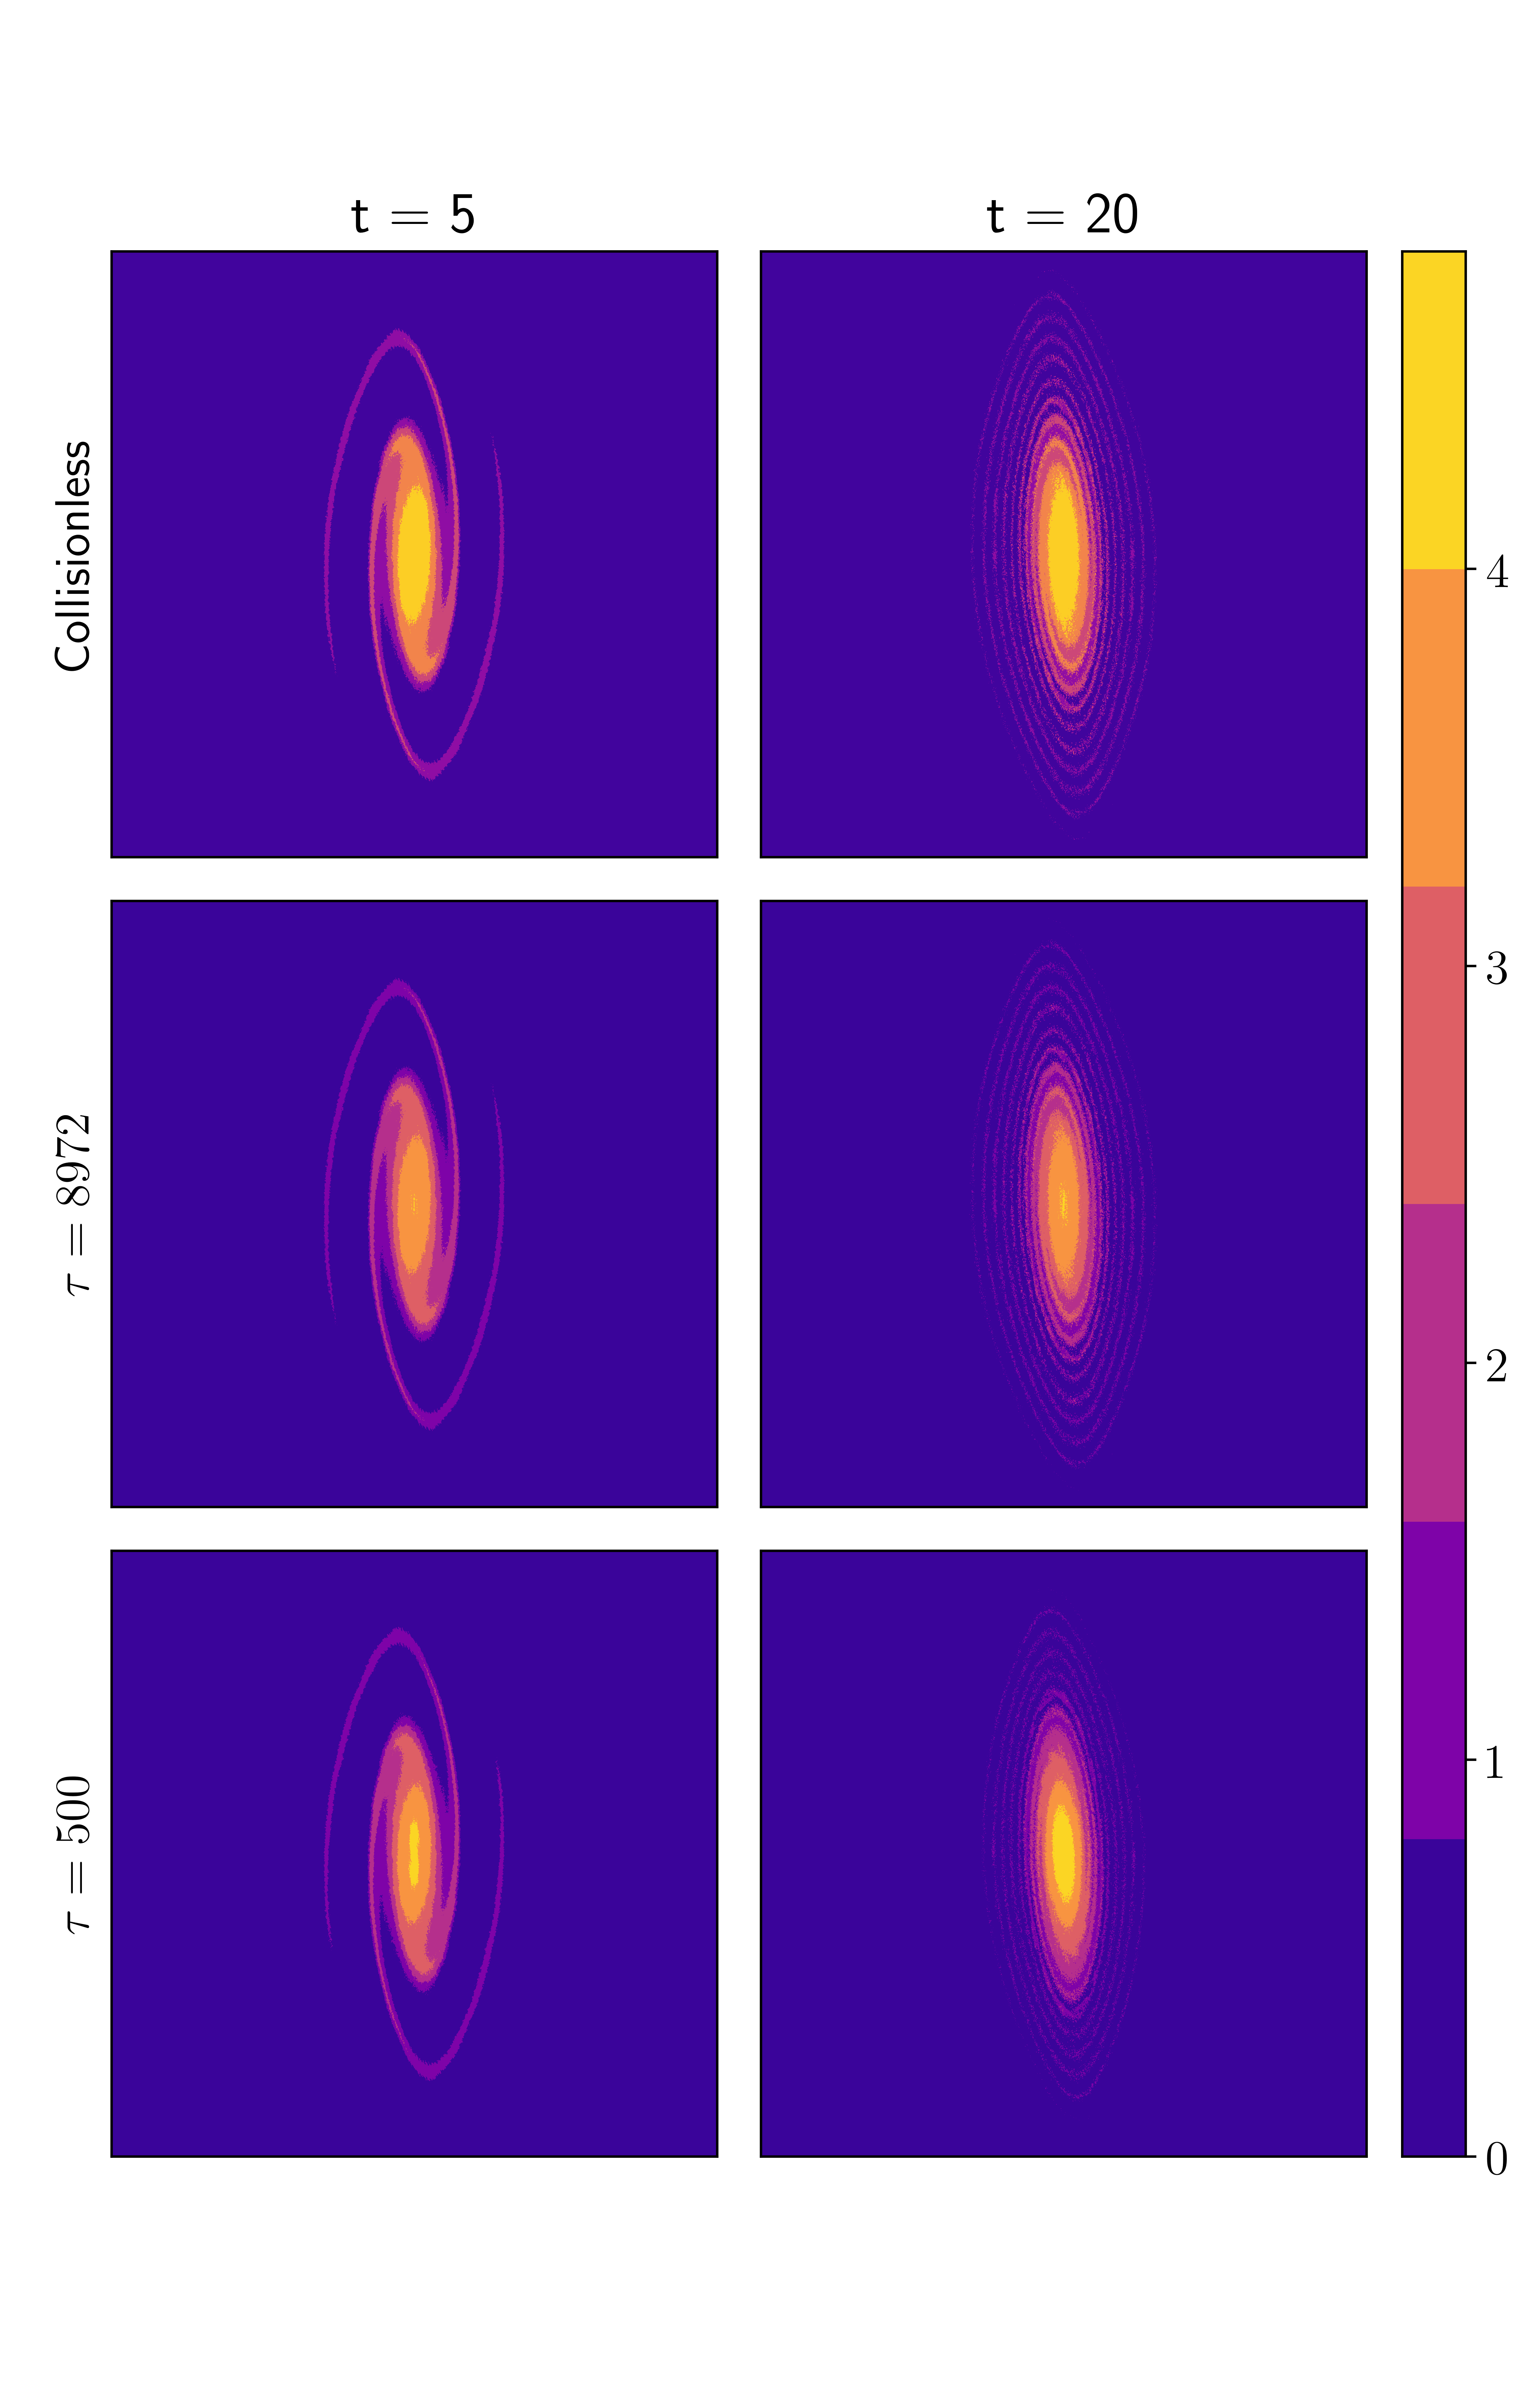
\includegraphics[scale=0.75]{images/gauss.png} %TODO cambiar color algo que funcione a escala de grices.
    \caption{Numerical test of Landau dampening for Gaussian initial conditions. We ran simulations with different values of $\tau$. All units are simulation units and have not being scaled for any astrophysical system in particular. It is easy to observe the thin arm structure mentioned in section \ref{sec: test_gauss}}
    \label{fig: Gauss_test}
\end{figure}



\subsection{Test II: Jeans Instability}
We initialize the phase space grid with a uniform density along with a periodic perturbation and a Gaussian velocity profile:
\begin{equation}
f(x,v,t = 0) = \frac{\bar{\rho}}{(2\pi \sigma^2)^{1/2}} \exp(-\frac{v^2}{2 \sigma}) (1 + A\cos(kx)) 
\end{equation} 

TODO

\section{Conclusions}

TODO

\section*{Acknowledgements}

TODO

%%%%%%%%%%%%%%%%%%%%%%%%%%%%%%%%%%%%%%%%%%%%%%%%%%

%%%%%%%%%%%%%%%%%%%% REFERENCES %%%%%%%%%%%%%%%%%%

% The best way to enter references is to use BibTeX:

\bibliographystyle{mnras}
\bibliography{bibTes} % if your bibtex file is called example.bib


%%%%%%%%%%%%%%%%%%%%%%%%%%%%%%%%%%%%%%%%%%%%%%%%%%

%%%%%%%%%%%%%%%%% APPENDICES %%%%%%%%%%%%%%%%%%%%%

\appendix

%%%%%%%%%%%%%%%%%%%%%%%%%%%%%%%%%%%%%%%%%%%%%%%%%%


% Don't change these lines
\bsp	% typesetting comment
\label{lastpage}
\end{document}

% End of mnras_template.tex

